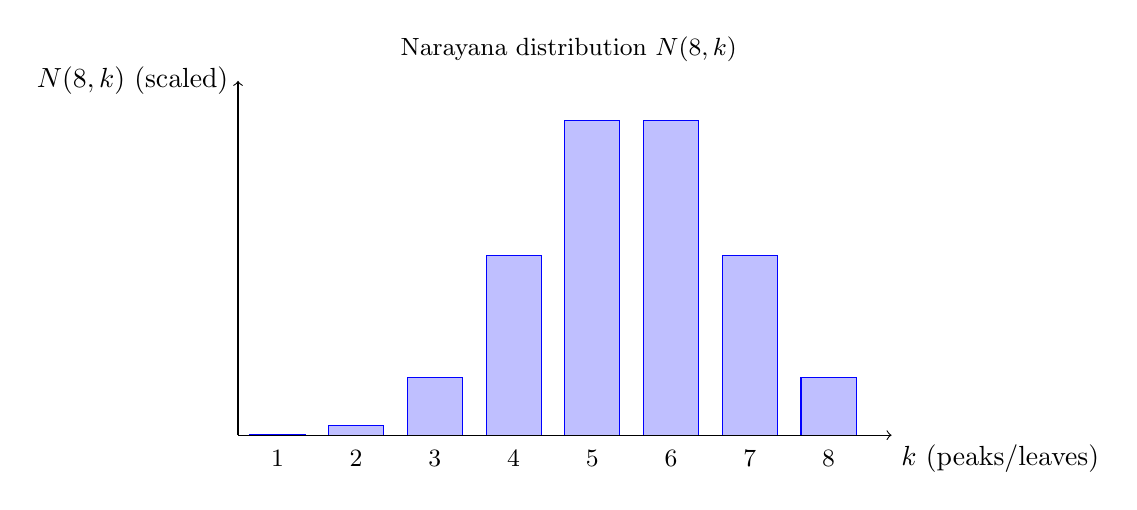
\begin{tikzpicture}[scale=1.0]
  % Hard-coded N(8,k) values for k=1..8: 1,14,84,264,462,462,264,84 (symmetric)
  \def\maxv{462}
  \foreach [count=\i] \v in {1,14,84,264,462,462,264,84} {
    % Height scaled into [0,4]
    \pgfmathsetmacro{\h}{4.0*\v/\maxv}
    % x-position of the bar center
    \pgfmathsetmacro{\x}{\i}
    % Draw bar
    \draw[fill=blue!25,draw=blue] ({\x-0.35},0) rectangle ({\x+0.35},\h);
    % k label below each bar
    \node at (\x,-0.3) {\small \i};
  }

  % Axes
  \draw[->] (0.5,0) -- (8.8,0) node[below right] {$k$ (peaks/leaves)};
  \draw[->] (0.5,0) -- (0.5,4.5) node[left] {$N(8,k)$ (scaled)};

  % Title
  \node at (4.7,4.9) {\small Narayana distribution $N(8,k)$};
\end{tikzpicture}
